% THIS DOCUMENT IS TAILORED TO REQUIREMENTS FOR SCIENTIFIC COMPUTING.  IT
% SHOULDN'T BE USED FOR NON-SCIENTIFIC COMPUTING PROJECTS
\documentclass[12pt]{article}

\usepackage{amsmath, mathtools}
\usepackage{amsfonts}
\usepackage{amssymb}
\usepackage{graphicx}
\graphicspath{{../assets}} % Bring in the assets

\usepackage{colortbl}
\usepackage{xr}
\usepackage{hyperref}
\usepackage{longtable}
\usepackage{xfrac}
\usepackage{tabularx}
\usepackage{float}
\usepackage{siunitx}
\usepackage{booktabs}
\usepackage{caption}
\usepackage{pdflscape}
\usepackage{afterpage}

\usepackage{tikz}
\usepackage{varwidth}
\usetikzlibrary{shapes,arrows,cd,babel,arrows.meta,graphs,graphdrawing}
\usegdlibrary {layered}

% Credit to Gabriel Devenyi for this bibliography cfg:
% github.com/gdevenyi/mcmaster.latex
\usepackage[ style=numeric-comp, backend=biber, sorting=none, backref=true,
  maxnames=99, alldates=iso, seconds=true ]{biblatex} % bibliography
\addbibresource{../references.bib}

%\usepackage{refcheck}

\hypersetup{
    bookmarks=true,    % show bookmarks bar?
    colorlinks=true,   % false: boxed links; true: colored links
    linkcolor=red,     % color of internal links (change box color with linkbordercolor)
    citecolor=green,   % color of links to bibliography
    filecolor=magenta, % color of file links
    urlcolor=cyan      % color of external links
}
\usepackage{cleveref}


% Force todonotes to play nicely in other floats: credits to https://tex.stackexchange.com/a/402075
\usepackage{marginnote}
\renewcommand{\marginpar}{\marginnote}

%% Comments

\usepackage{color}

\newif\ifcomments\commentstrue %displays comments
%\newif\ifcomments\commentsfalse %so that comments do not display

\ifcomments
\newcommand{\authornote}[3]{\textcolor{#1}{[#3 ---#2]}}
\newcommand{\todo}[1]{\textcolor{red}{[TODO: #1]}}
\else
\newcommand{\authornote}[3]{}
\newcommand{\todo}[1]{}
\fi

\newcommand{\wss}[1]{\authornote{blue}{SS}{#1}} 
\newcommand{\plt}[1]{\authornote{magenta}{TPLT}{#1}} %For explanation of the template
\newcommand{\an}[1]{\authornote{cyan}{Author}{#1}}

%% Common Parts

\newcommand{\progname}{BeamBending}
\newcommand{\authname}{\small{\textit{Team Drasil}}\\Jason Balaci}
\newcommand{\authinitials}{JB}

\usepackage{hyperref}
\hypersetup{colorlinks=true, linkcolor=blue, citecolor=blue, filecolor=blue,
            urlcolor=blue, unicode=false}
\urlstyle{same}

\usepackage{newunicodechar}

\newunicodechar{Ȧ}{$\dot{A}$}


% For easy change of table widths
\newcommand{\colZwidth}{1.0\textwidth}
\newcommand{\colAwidth}{0.13\textwidth}
\newcommand{\colBwidth}{0.82\textwidth}
\newcommand{\colCwidth}{0.1\textwidth}
\newcommand{\colDwidth}{0.05\textwidth}
\newcommand{\colEwidth}{0.8\textwidth}
\newcommand{\colFwidth}{0.17\textwidth}
\newcommand{\colGwidth}{0.5\textwidth}
\newcommand{\colHwidth}{0.28\textwidth}

% Used so that cross-references have a meaningful prefix
\newcounter{defnum} %Definition Number
\newcommand{\dthedefnum}{GD\thedefnum}
\newcommand{\dref}[1]{GD\ref{#1}}
\newcounter{datadefnum} %Datadefinition Number
\newcommand{\ddthedatadefnum}{DD\thedatadefnum}
\newcommand{\ddref}[1]{DD\ref{#1}}
\newcounter{theorynum} %Theory Number
\newcommand{\tthetheorynum}{T\thetheorynum}
\newcommand{\tref}[1]{TM\ref{#1}}
\newcounter{tablenum} %Table Number
\newcommand{\tbthetablenum}{T\thetablenum}
\newcommand{\tbref}[1]{TB\ref{#1}}
\newcounter{assumpnum} %Assumption Number
\newcommand{\atheassumpnum}{P\theassumpnum}
\newcommand{\aref}[1]{A\ref{#1}}
\newcounter{goalnum} %Goal Number
\newcommand{\gthegoalnum}{P\thegoalnum}
\newcommand{\gsref}[1]{GS\ref{#1}}
\newcounter{instnum} %Instance Number
\newcommand{\itheinstnum}{IM\theinstnum}
\newcommand{\iref}[1]{IM\ref{#1}}
\newcounter{reqnum} %Requirement Number
\newcommand{\rthereqnum}{P\thereqnum}
\newcommand{\rref}[1]{R\ref{#1}}
\newcounter{nfrnum} %NFR Number
\newcommand{\rthenfrnum}{NFR\thenfrnum}
\newcommand{\nfrref}[1]{NFR\ref{#1}}
\newcounter{lcnum} %Likely change number
\newcommand{\lthelcnum}{LC\thelcnum}
\newcommand{\lcref}[1]{LC\ref{#1}}

\usepackage{fullpage}

\newcounter{theorycounter}
\newcommand{\deftheory}[9][Not Applicable]
{
\newpage
\noindent \rule{\textwidth}{0.5mm}

\paragraph{RefName: } \refstepcounter{theorycounter}TM\thetheorycounter \phantomsection 
\label{#2}

\paragraph{Label:} #3

\noindent \rule{\textwidth}{0.5mm}

\paragraph{Equation:}

#4

\paragraph{Description:}

#5

\paragraph{Notes:}

#6

\paragraph{Source:}

#7

\paragraph{Ref.\ By:}

#8

\paragraph{Preconditions for TM\thetheorycounter{}:}
\label{#2_precond}

#9

\paragraph{Derivation for TM\thetheorycounter{}:}
\label{#2_deriv}

#1

\noindent \rule{\textwidth}{0.5mm}

}

\begin{document}


% START : TODO LIST
% Only show it if the "comments" flag is enabled
\ifcomments
    \todototoc
    \listoftodos
    \newpage
\fi
% END   : TODO LIST

%%%%%%%%%%%%%%%%%%%%%%%%%%%%%%%%%%%%%%%%%%%%%%%%%%%%%%%%%%%%%%%%%%%%%%%%%%%%%%%
% Title
%%%%%%%%%%%%%%%%%%%%%%%%%%%%%%%%%%%%%%%%%%%%%%%%%%%%%%%%%%%%%%%%%%%%%%%%%%%%%%%

\title{Software Requirements Specification for \progname: examining a beam
    bending under load.}
\author{\authname}
\date{\today}

\maketitle

~\newpage

\pagenumbering{roman}

\tableofcontents

~\newpage

%%%%%%%%%%%%%%%%%%%%%%%%%%%%%%%%%%%%%%%%%%%%%%%%%%%%%%%%%%%%%%%%%%%%%%%%%%%%%%%
% Revision History
%%%%%%%%%%%%%%%%%%%%%%%%%%%%%%%%%%%%%%%%%%%%%%%%%%%%%%%%%%%%%%%%%%%%%%%%%%%%%%%

\section*{Revision History}

\begin{tabularx}{\textwidth}{p{3cm}p{2cm}X}
    \toprule {\bf Date} & {\bf Version} & {\bf Notes}                           \\
    \midrule
    Jan. 25, 2023       & 0.0.0         & Template imported.                    \\
    Jan. 25, 2023       & 0.1.0         & Preliminary information added.        \\
    Jan. 25, 2023       & 0.1.1         & Table of units added.                 \\
    Jan. 25, 2023       & 0.1.2         & Table of symbols added.               \\
    Jan. 25, 2023       & 0.1.3         & Refining above tables.                \\
    Jan. 25, 2023       & 0.2.0         & Refined introduction.                 \\
    Jan. 25, 2023       & 0.3.0         & Refining GSD, SSD, TMs, and IMs.      \\
    Feb. 4, 2023        & 0.4.0         & Work on things other than the models. \\
    Feb. 5, 2023        & 0.5.0         & Refining models (again).              \\
    Feb. 6, 2023        & 0.6.0         & Complete rough draft.                 \\
    \bottomrule
\end{tabularx}

~\newpage

%%%%%%%%%%%%%%%%%%%%%%%%%%%%%%%%%%%%%%%%%%%%%%%%%%%%%%%%%%%%%%%%%%%%%%%%%%%%%%%
% Reference Material
%%%%%%%%%%%%%%%%%%%%%%%%%%%%%%%%%%%%%%%%%%%%%%%%%%%%%%%%%%%%%%%%%%%%%%%%%%%%%%%

\section{Reference Material}

This section records information for easy reference.

\subsection{Table of Units}

Throughout this document SI (Syst\`{e}me International d'Unit\'{e}s) is employed
as the unit system.  In addition to the basic units, several derived units are
used as described below.  For each unit, the symbol is given followed by a
description of the unit and the SI name. ~\newline

\begin{center}
    \renewcommand{\arraystretch}{1.2}
    \noindent \begin{tabular}{l l l}
        \toprule
        \textbf{symbol} & \textbf{unit} & \textbf{SI} \\
        \midrule
        \si{\metre}     & length        & metre       \\
        \si{\kilo\gram} & mass          & gram        \\
        \si{\pascal}    & pressure      & pascal      \\
        \si{\radian}    & angle         & radian      \\
        \si{\newton}    & force         & newton      \\
        \bottomrule
    \end{tabular}\\
\end{center}

\noindent{}Note that we will also often use:

\begin{itemize}

    \item ``gigapascals'' (a unit of pressure, denoted by \si{\giga\pascal},
          where \(\si{\giga\pascal}=10^{9}\si{\pascal}\)),

    \item ``kilonewtons'' (a unit of force, denoted by \si{\kilo\newton}, where
          \(\si{\kilo\newton}=10^{3}\si{\newton}\)), and

    \item ``millimetres'' (a unit of length, denoted by \si{\milli\metre}, where
          \(\si{\milli\metre}=10^{-5}\si{\metre}\)).

\end{itemize}

\subsection{Table of Symbols}

The table that follows summarizes the symbols used in this document along with
their units.  The choice of symbols was made to be consistent with the heat
transfer literature and with existing documentation for solar water heating
systems.  The symbols are listed in alphabetical order.

\renewcommand{\arraystretch}{1.2}
\noindent
\begin{longtable*}{l l p{12cm}}
    \toprule
    \textbf{symbol} & \textbf{unit} & \textbf{description}\\
    \midrule
    \(L\) & \si{\metre} & abstract length of the beam \\
    \(E\) & \si{\giga\pascal} & abstract Young's modulus (beam material modulus of elasticity) \\
    \(I\) & \(\si{\metre{}}^{4}\) & abstract moment of inertia \\
    \(L_{B}\) & \si{\metre} & user-defined length of the beam \\
    \(E_{B}\) & \si{\giga\pascal} & user-defined Young's modulus (beam material modulus of elasticity) \\
    \(I_{B}\) & \(\si{\metre{}}^{4}\) & user-defined moment of inertia of a cross-section of the beam \\
    \(w_B(x)\) & \si{\kilo\newton} & user-defined definition of the force of the load applied at a specific point along the beam \\
    \(x\) & \si{\metre} & distance of an arbitrary point along the beam, from the far left-side (at the pinned support) \\
    \(w(x)\) & \si{\kilo\newton} & hypothetical force of the load applied at a specific point along the beam \\
    \(\mathit{Pinned}\) & \si{\metre} & 1-dimensional position of the pinned support \\
    \(\mathit{Roller}\) & \si{\metre} & 1-dimensional position of the roller support \\
    \(R_{\mathit{Pinned}}\) & \si{\kilo\newton} & reaction of the pinned support under loaded beam \\
    \(R_{\mathit{Roller}}\) & \si{\kilo\newton} & reaction of the roller support under loaded beam \\
    \(\theta{}_{\mathit{Pinned}}\) & \si{\radian} & slope of the angle between the beam and the pinned support under load \\
    \(\theta{}_{\mathit{Roller}}\) & \si{\radian} & slope of the angle between the beam and the roller support under load \\
    \(y(x)\) & \si{\milli\metre} & deflection of a hypothetical loaded beam at a specific point along it \\
    \(y_{B}(x)\) & \si{\milli\metre} & deflection of the loaded beam at a specific point along it \\
    \bottomrule
\end{longtable*}

\subsection{Abbreviations and Acronyms}

\renewcommand{\arraystretch}{1.2}

\begin{center}
    \begin{tabular}{l l}
        \toprule
        \textbf{symbol} & \textbf{description}                \\
        \midrule
        A               & Assumption                          \\
        BVP             & Boundary Value Problem              \\
        DD              & Data Definition                     \\
        GD              & General Definition                  \\
        GS              & Goal Statement                      \\
        IM              & Instance Model                      \\
        LC              & Likely Change                       \\
        PS              & Physical System Description         \\
        R               & Requirement                         \\
        SRS             & Software Requirements Specification \\
        \progname{}     & Beam Bending                        \\
        TM              & Theoretical Model                   \\
        \bottomrule
    \end{tabular}
\end{center}

\subsection{Mathematical Notation}

The common mathematical notation used in Canadian undergraduate-level
mathematics will be used throughout this document.

\newpage

\pagenumbering{arabic}

%%%%%%%%%%%%%%%%%%%%%%%%%%%%%%%%%%%%%%%%%%%%%%%%%%%%%%%%%%%%%%%%%%%%%%%%%%%%%%%
% Introduction
%%%%%%%%%%%%%%%%%%%%%%%%%%%%%%%%%%%%%%%%%%%%%%%%%%%%%%%%%%%%%%%%%%%%%%%%%%%%%%%

\section{Introduction}

For any load-carrying structure, beams safely distribute the stress of the load
to the foundations of the structure. Unlike flooring in residential homes, we
expect the beds of industrial-strength mechanical tools and bridges to, within
reason, be vertically and horizontally flexible, reacting to imposed load such
that they may hold with minimal columns. \textit{Simply supported} beams are one
type of beam that are commonly found in bridges and beds of machine tools. It is
important to understand how beams will react under load or else we risk damaging
structures, floor bending (making inhabitants feel unsafe), or damaging loads.
We may use software to analyze the beams reaction under various loading
scenarios. We call the software that performs this: ``BeamBending.''

This document aims to develop a general scheme for understanding the reaction of
a simply supported beam to imposed load under simplified conditions. This
section aims to provide an overview of the Software Requirements Specification
(SRS) for the ``BeamBending'' problem, discussing the scope and purpose of the
work.

\subsection{Purpose of Document}

The purpose of this document is to provide the reader with a well-derived,
verifiable explanation of a solution to the ``beam bending'' problem. The
document provides sufficient information such that a related software artifact
may be constructed. The produced software artifact has an ``increased'' degree
of confidence in reliability and correctness by being traceable to and derived
by these defined software requirements specifications. As such, a large focus on
the development of this document is to have the domain knowledge captured and
adequately codified such that the origins of fragments of code may be verified,
up to development choices (e.g., language, tooling, etc.).

\subsection{Scope of Requirements}
\label{ssec_scope}

The requirements analyze the ``problem'' (as defined in \Cref{Sec_pd}) and
related ``solution'' under the assumption of the Euler-Bernoulli Beam Theory
\cite{EulerBernoulliWiki} in a 2-dimensional space for a prismatic beam.

\subsection{Characteristics of Intended Reader}
\label{sec_IntendedReader}

Readers of this document should at least have an understanding of:
\begin{itemize}
    \item at least a first-year university level physics concepts, such as
          ``force,'' ``mass,'' ``inertia,'' ``elasticity,'' and ``units,''
    \item first-year university level linear algebra and calculus concepts, such
          as derivatives, integration, continuous functions, and vectors.
\end{itemize}

However, it is preferred that users have at least a second-year university level
understand of physics and calculus concepts to confidently audit the derivation
of the instance models.

Should this document be used for non-trivial, non-educational purposes, this
document should strictly be read and used by those appropriately licensed and
well-versed in software and civil engineering.

\subsection{Organization of Document}

This document follows the SRS template as specified by Smith and Lai
\cite{SmithAndLai2005}. If you are already familiar with the SRS template, the
author's recommended, but not required, reading order is as follows:

\begin{itemize}
    \item \nameref{Sec_pd},
    \item \nameref{sssec_goals},
    \item \nameref{sec_IntendedReader},
    \item \nameref{ssec_scope},
    \item \nameref{sec_gsd},
    \item \nameref{sec_assumpt},
    \item \nameref{sec_ssd}, and, finally,
    \item \nameref{sec_instance} to \nameref{sec_theoretical}.
\end{itemize}

\noindent{}The other material is referential and may be read as needed.

\newpage

%%%%%%%%%%%%%%%%%%%%%%%%%%%%%%%%%%%%%%%%%%%%%%%%%%%%%%%%%%%%%%%%%%%%%%%%%%%%%%%
% General System Description
%%%%%%%%%%%%%%%%%%%%%%%%%%%%%%%%%%%%%%%%%%%%%%%%%%%%%%%%%%%%%%%%%%%%%%%%%%%%%%%

\section{General System Description}
\label{sec_gsd}

This section provides general information about the system so that the next
section will be easier to digest. It identifies the interfaces between the
system and its environment, describes the user characteristics, and lists the
system constraints.

\subsection{System Context}

\Cref{Fig_SystemContext} represents an abstract view of the software. The
rectangular node represents the ``BeamBending'' software itself, whilst circular
nodes represent external entities interacting with the ``BeamBending'' software.
The abstract view is that a user would provide input information (beam and load
specifications) to the software, which would use a provided, external, Boundary
Value Problem (BVP) solver to process the inputs, and output the expected
deflection curve.

\begin{figure}[h!]
    \begin{center}
        \begin{tikzpicture}
            % draw the nodes
            \node [draw,circle] (I) at (-6, 0) {\textbf{User}};
            \node [draw,rectangle] (BB) at (0, 0) {\textbf{BeamBending}};
            \node [draw,circle] (O) at (6, 0) {\textbf{User}};
            \node [draw,circle] (E) at (0,-4) {\parbox{1.5cm}{\center\textbf{BVP Solver}}};

            % draw the arrows between the nodes
            \draw [->] (I) -- (BB) node[midway,above] {\parbox{3cm}{\center\textbf{Input}:\newline{}beam \& load specifications.}};
            \draw [->] (BB) -- (O) node[midway,above] {\parbox{3cm}{\center\textbf{Output}:\newline{}deflection curve.}};
            \draw [<->] (E) -- (BB) node[midway,left] {\parbox{2.5cm}{\center{}Solver provides BVP solutions on demand.}};
        \end{tikzpicture}
    \end{center}
    \caption{System Context}
    \label{Fig_SystemContext}
\end{figure}

\begin{itemize}
    \item User Responsibilities:
          \begin{itemize}

              \item Providing material properties of the beam, taking required
                    units, assumptions, and applicability of the beam into
                    consideration.

              \item Providing an explanation of the imposed load as a function
                    of the distance from the leftward pinned support.

              \item Interpret the output of the program taking this SRS document
                    into consideration and use an audited and reliable copy of a
                    software related to this SRS.

          \end{itemize}

    \item \progname{} Responsibilities:
          \begin{itemize}

              \item Detect data type mismatches, such as a string of characters
                    instead of a floating point number.

              \item Evaluate applicability of the input arguments to the
                    proposed ``solution'' outlined in this document, such as
                    numbers being above a certain threshold with respect to
                    others (e.g., the number of sampling points must be a
                    positive, non-zero, number).

              \item Calculate the imposed loading and resultant deflection at
                    every desired sampling point, the angles of rotation between
                    the beam and the respective supports, the force reactions at
                    the supports, and the movement of the beam in the horizontal
                    direction.

          \end{itemize}
\end{itemize}

\subsection{User Characteristics}
\label{SecUserCharacteristics}

The user of this software should be a civil engineer or equivalent, and have a
working understanding of the deflection of beams, shear forces, bending moments,
and related concepts. If applied in educational purposes, only an understanding
of first-year physics and calculus is required to generally understand the
program and simulate a simply-supported beam across various scenarios.

\subsection{System Constraints}

The final software should be built using Drasil to encode the problem and
generate a problem using a BVP solver. There are no other system constraints.
However, it should be noted that the usage of Drasil does impose the limitations
of Drasil onto the produced software and SRS documents. One notable limitation
is the inability to input general expressions into Drasil-generated programs. As
such, the ``user-defined'' loading function, \(w_{B}(x)\), will need to be
hard-coded into both this SRS document and the software. However, changing the
source for both is relatively straightforward and simple thanks to Drasil.

\newpage

%%%%%%%%%%%%%%%%%%%%%%%%%%%%%%%%%%%%%%%%%%%%%%%%%%%%%%%%%%%%%%%%%%%%%%%%%%%%%%%
% Specific System Description
%%%%%%%%%%%%%%%%%%%%%%%%%%%%%%%%%%%%%%%%%%%%%%%%%%%%%%%%%%%%%%%%%%%%%%%%%%%%%%%

\section{Specific System Description}
\label{sec_ssd}

This section first presents the problem description, which gives a high-level
view of the problem to be solved.  This is followed by the solution
characteristics specification, which presents the assumptions, theories,
definitions and finally the instance models.

\subsection{Problem Description}
\label{Sec_pd}

\progname{} is intended to solve for the deflection a beam experiences given a
load-application function and properties of the beam.

\subsubsection{Terminology and  Definitions}

This subsection provides a list of terms that are used in the subsequent
sections and their meaning, with the purpose of reducing ambiguity and making it
easier to correctly understand the requirements:

\begin{itemize}

    \item beam: structural components intended to carry loads perpendicularly to
          their ``long'' axis\nc{},

    \item pinned support: a structural support that allows for rotation but
          neither vertical nor horizontal movement\nc{},

    \item roller support: a structural support that allows for rotation and
          horizontal movement, but not vertical movement\nc{},

    \item simply supported beam: a beam that has a pinned support on one end,
          and a roller support on the other\nc{},

    \item load: an applied force to a structure\nc{},

    \item deflection: the amount that a structural component is displaced due to
          deformation under load\nc{},

    \item shear forces: unaligned opposed forces acting on an object (e.g.,
          shears or scissors) that can result in tearing\nc{},

    \item bending moment: the internal reaction of a structural element when an
          external force is imposed and bends it\nc{},

    \item Young's modulus (modulus of elasticity): the measure of lengthwise
          stiffness of an element as a force is applied lengthwise\nc{}, and

    \item moment of inertia: torque required for angular acceleration\nc{}.

\end{itemize}

\subsubsection{Physical System Description}
\label{sec_phySystDescrip}

An ``at-rest'' view of the physical system of \progname{}, as shown in
\Cref{beam_bending_diagram}, includes the following elements:

\begin{itemize}

    \item a slender beam,

    \item a pinned support, and

    \item a roller support.

\end{itemize}

\begin{figure}[H]
    \begin{center}
        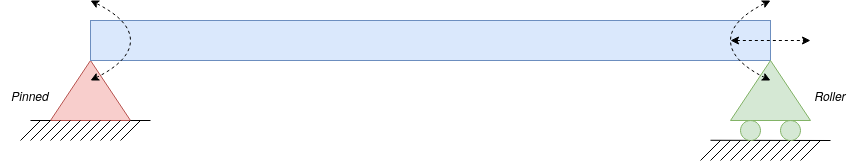
\includegraphics[width=0.9\textwidth]{temp/beam_bending_diagram.drawio.png}
        \caption{\label{beam_bending_diagram} Diagram of a Simply Supported Beam}
    \end{center}
\end{figure}

\Cref{beam_bending_diagram} shows the physical system at equilibrium. A slender
beam is supported by a pinned support and a roller support. For the sake of
following convention, the pinned support is placed on the left side of the beam,
while the roller support is on the right. Additionally, when thinking of
distance along the beam, we think of it as a distance from the pinned support on
the left-hand side. As shown in \Cref{beam_bending_diagram}, the pinned support
allows for rotational movements about the support tip, while the roller support
also allows for some horizontal movement along the roller. When the beam is
loaded, the roller support allows for tensile/compressive changes in the beam
(which would alter the length of the beam).

The physical system described in \progname{} examines
\Cref{beam_bending_diagram} under an inputted general loading function. As such,
the ``whole'' system is as per \Cref{beam_bending_diagram_annotated},
containing:

\begin{itemize}

    \item[\textbf{PS1}:] a slender beam,

    \item[\textbf{PS2}:] a pinned support,

    \item[\textbf{PS3}:] a roller support, and

    \item[\textbf{PS4}:] an applied load.

\end{itemize}

\begin{figure}[H]
    \begin{center}
        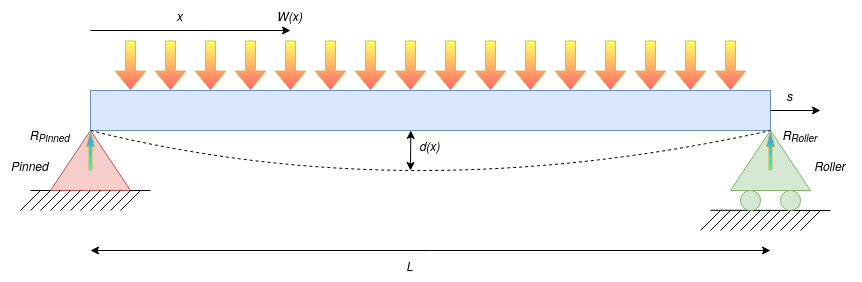
\includegraphics[width=0.9\textwidth]{temp/beam_bending_diagram_annotated.drawio.png}
        \caption{\label{beam_bending_diagram_annotated} Diagram of a Simply Supported Beam Under Load}
    \end{center}
\end{figure}

However, note that at the ``boundaries'' (the support tips), the beam may not
have vertical deflection, and similarly has zero bending moment at the tips.
Additionally, it should be noted that the beam is considered
\textit{determinant}.

\subsubsection{Goal Statements}
\label{sssec_goals}

\noindent{}Given constant length, modulus of elasticity, and moment of inertia
across cross-sections of the beam, and the applied load on the beam as a
function from the distance of the leftward pinned support, the goal statements
are:

\begin{itemize}

    \item[\refstepcounter{goalnum}\textbf{GS\thegoalnum{}}\label{deflection}:]
        Calculate the deflection of the beam under load.

    \item[\refstepcounter{goalnum}\textbf{GS\thegoalnum{}}\label{reaction}:]
        Calculate the reaction of the supports under load.

\end{itemize}

\subsection{Solution Characteristics Specification}

The instance models that govern \progname{} are presented in
Subsection~\ref{sec_instance}.  The information to understand the meaning of the
instance models and their derivation is also presented, so that the instance
models can be verified.

\subsubsection{Assumptions}
\label{sec_assumpt}

This section simplifies the original problem and helps in developing the
theoretical model by filling in the missing information for the physical system.
The numbers given in the square brackets refer to the Theoretical Model (TM),
General Definition (GD), Data Definition (DD), Instance Model (IM), or Likely
Change (LC), in which the respective assumption is used.

\newcommand{\assume}[2]{\refstepcounter{assumpnum}\item[\textbf{A\theassumpnum{}}\label{#1}:] #2}

\begin{itemize}

    \assume{world_dimension}{The ``world'' model is 2-dimensional, observing the
        instant a load is applied on the beam.}

    \assume{beam_slender}{The beam is ``slender'' (has a length to height ratio
        greater than \(10\) to \(1\)).}

    \item \textit{The beam is prismatic.}
          \begin{itemize}
              \assume{beam_uniform_cross_section}{The beam has a uniform cross-section.}
              \assume{beam_straight_faces}{The beam is straight/flat within a
                  reasonable tolerance.}
          \end{itemize}

          \assume{beam_moment_inertia_constant}{The beam has a constant moment of
              inertia.}

          \assume{beam_vertical_elastic}{The beam experiences vertical linear-elastic
              load.}

          \assume{beam_modulus_constant}{The beam's modulus of elasticity is constant
              along the beam.}

          \assume{beam_deflection}{Only relatively small deflections will be examined
              (whereby the maximum deflection is at most \(10\%\) of the beam's
              length).}

          \assume{deflection_differentiable}{The hypothetical deflection function
              should belong to at least the class of functions that are differentiable
              4 times on \([0, L]\).}

          \assume{loading_integrable}{The loading function should belong to at least
              the class of functions that are integrable 4 times on \([0, L]\).}

\end{itemize}

\subsubsection{Theoretical Models}
\label{sec_theoretical}

This section focuses on the general equations and laws that \progname{} is based
on.

\noindent
\deftheory
% #2 refname of theory
{TM:PC}
% #3 label
{Curvature of a Plane}
% #4 equation
{
    \[\frac{1}{\rho} = \frac{\frac{d^{2}y}{dx^{2}}}{(1+(\frac{dy}{dx})^{2})^{\frac{3}{2}}}\]
}
% #5 description
{ From elementary calculus, the curvature of a plane curve at a point \(Q(x,y)\)
    of a curve may be expressed by the above equation, where
    \cite{BeerJohnston1981}:

    \begin{itemize}
        \item \(\rho\) is the radius of curvature,
        \item \(y\) is the vertical component of the point, and
        \item \(x\) is the horizontal component of the point.
    \end{itemize}
}
% #6 Notes
{
    None.
}
% #7 Source
{
    \cite{BeerJohnston1981}
}
% #8 Referenced by
{
    \tref{TM:OREC}
}
% #9 Preconditions
{
    None.
}
% #1 derivation - not applicable by default
{
}

\noindent
\deftheory
% #2 refname of theory
{TM:PBPBA}
% #3 label
{Prismatic Beam Pure Bending into Arc}
% #4 equation
{
    \[\frac{1}{\rho} = \frac{M(x)}{EI}\]
}
% #5 description
{ For a beam, the reciprocal of the radius of curvature is a ratio of the
    bending moment ($M(x)$) to the flexural rigidity ($EI$). }
% #6 Notes
{
    None.
}
% #7 Source
{
    \cite{BeerJohnston1981}
}
% #8 Referenced by
{
    \tref{TM:OREC}
}
% #9 Preconditions
{
    None.
}
% #1 derivation - not applicable by default
{
}

\noindent
\deftheory
% #2 refname of theory
{TM:OREC}
% #3 label
{ODE Relationship of an Elastic Curve}
% #4 equation
{
    \[\frac{d^{2}y}{dx^{2}} = \frac{M(x)}{EI}\]
}
% #5 description
{
}
% #6 Notes
{
    None.
}
% #7 Source
{
    \cite{BeerJohnston1981}
}
% #8 Referenced by
{
    \tref{TM:EBBDE}
}
% #9 Preconditions
{
    None.
}
% #1 derivation - not applicable by default
{ Starting with \tref{TM:PC}:

    \[\frac{1}{\rho} = \frac{\frac{d^{2}y}{dx^{2}}}{(1+(\frac{dy}{dx})^{2})^{\frac{3}{2}}}\]

    We may recognize that in the context of an abstract prismatic beam, the slope
    \(\frac{dy}{dx}\) is relatively ``small'' (\aref{beam_deflection}). Similarly,
    its square is also small. Considering it negligible, we may drop it:

    \[\frac{1}{\rho} = \frac{d^{2}y}{dx^{2}}\]

    However, substituting \(\frac{1}{\rho}\) from \tref{TM:PBPBA}, we obtain:

    \[\frac{d^{2}y}{dx^{2}} = \frac{M(x)}{EI}\]
}

\noindent
\deftheory
% #2 refname of theory
{TM:EBBDE}
% #3 label
{Euler-Bernoulli Beam Deflection Equation}
% #4 equation
{
    \[EI\frac{d^{4}y}{dx^{4}}=w(x)\]
}
% #5 description
{ The above equation describes the relationship between a beam's deflection
    (\(y(x)\)) and the applied load (\(w(x)\)) for any point along the beam
    (\(x\)). Notably,

    \begin{itemize}
        \item $y(0)=0$,
        \item $y(L)=0$,
        \item $\frac{d^{2}}{dx^2} y(0) = 0$, and
        \item $\frac{d^{2}}{dx^2} y(L) = 0$
    \end{itemize}

    because the beam is simply supported (fixed at both ends implying no
    vertical movement), and hence the moments at the ends are 0. }
% #6 Notes
{ None. }
% #7 Source
{
    \cite{BeerJohnston1981,EulerBernoulliWiki}
}
% #8 Referenced by
{
    \iref{im_deflection}
}
% #9 Preconditions
{ None. }
% #1 derivation - not applicable by default
{ When a prismatic beam supports an applied loading, (\(w(x)\)), its elastic
    curve is governed by the fourth-order ODE found by integrating the equation
    found in \tref{TM:OREC} twice.
}

\newpage

\subsubsection{General Definitions}
\label{sec_gendef}

There are no general definitions.

\subsubsection*{Detailed derivation of simplified rate of change of temperature}

\subsubsection{Data Definitions}
\label{sec_datadef}

\noindent
\begin{minipage}{\textwidth}
    \renewcommand*{\arraystretch}{1.5}
    \begin{tabular}{| p{\colAwidth} | p{\colBwidth}|}
        \hline
        \rowcolor[gray]{0.9}
        Number      & DD\refstepcounter{datadefnum}\thedatadefnum \label{dd_loading_function} \\ \hline
        Label       & \bf Applied Load                                                        \\ \hline
        Symbol      & $w_{B}(x)$                                                              \\ \hline
        SI Units    & \si{\watt\per\square\metre}                                             \\ \hline
        Equation    & $w_{B}(x) = (x - \frac{L_B}{2})^{2}$                                    \\ \hline
        Description & $w_{B}(x)$ is the function describing the load applied along the beam.  \\
                    & $x$ is a point along the beam.                                          \\
                    & $L_B$ is the length of the beam.                                        \\ \hline
        Ref.\ By    & \iref{im_deflection}                                                    \\ \hline
    \end{tabular}
\end{minipage}\\

\subsubsection{Data Types}
\label{sec_datatypes}

The conventional data types used in undergraduate-level physics courses is
sufficient. As such, the specifications define no extra data types.

\subsubsection{Instance Models}
\label{sec_instance}

This section transforms the problem defined in Section~\ref{Sec_pd} into one
which is expressed in mathematical terms. It uses concrete symbols defined in
Section~\ref{sec_datadef} to replace the abstract symbols in the models
identified in Sections~\ref{sec_theoretical} and~\ref{sec_gendef}. Notably,
\gsref{deflection} is solved by \iref{im_deflection}.

%Instance Model 1

\noindent
\begin{minipage}{\textwidth}
    \renewcommand*{\arraystretch}{1.5}
    \begin{tabular}{| p{\colAwidth} | p{\colBwidth}|}
        \hline
        \rowcolor[gray]{0.9}
        Number      & IM\refstepcounter{instnum}\theinstnum{}\label{im_deflection}           \\ \hline
        Label       & \bf Beam Deflection                                                    \\ \hline
        Input       & $L_B$, $E_B$, $I_B$, $w_{B}(x)$                                        \\ \hline
        Output      & \(y_{B}(x)\) as the solution to the BVP defined as:                    \\
                    & \(E_{B}I_{B}\frac{d^{4}y_{B}}{dx^{4}}=w_{B}(x)\) where \(y_{B}(0)=0\),
        \(\frac{d^{2}y_{B}}{dx^{2}}(0)=0\), \(y_{B}(L_B)=0\), and
        \(\frac{d^{2}y_{B}}{dx^{2}}(L_B)=0\)                                                 \\ \hline
        Description & The above output is the solution of the above defined BVP.             \\
                    & $L_B$ is the beam's length.                                            \\
                    & $E_B$ is the beam's modulus of elasticity (Young's modulus).           \\
                    & $I_B$ is the beam's moment of inertia.                                 \\
                    & $w_{B}(x)$ is the function describing the load applied along the beam. \\
                    & $x$ is a point along the beam.                                         \\
                    & $y_{B}(x)$ is a function describing the deflection along the beam.     \\ \hline
        Sources     & \nc{}                                                                  \\ \hline
        Ref.\ By    &                                                                        \\ \hline
    \end{tabular}
\end{minipage}\\

\subsubsection*{Derivation of Beam Deflection:}

This model is a direct instantiation of \tref{TM:EBBDE} observed as a BVP for
the beam in question as provided by user inputs (i.e., with $L_B$, $E_B$, $I_B$,
$w_B$, $y_B$ substituted in).

\subsubsection{Input Data Constraints}
\label{sec_DataConstraints}

Table~\ref{TblInputVar} shows the data constraints on the input \& output
variables.  The column for physical constraints gives the physical limitations
on the range of values that can be taken by the variable.  The column for
software constraints restricts the range of inputs to reasonable values.  The
software constraints will be helpful in the design stage for picking suitable
algorithms.  The constraints are conservative, to give the user of the model the
flexibility to experiment with unusual situations.  The column of typical values
is intended to provide a feel for a common scenario.  The uncertainty column
provides an estimate of the confidence with which the physical quantities can be
measured.  This information would be part of the input if one were performing an
uncertainty quantification exercise.

The specification parameters in Table~\ref{TblInputVar} are listed in
Table~\ref{TblSpecParams}.

\begin{table}[!h]
    \caption{Input Variables} \label{TblInputVar}
    \renewcommand{\arraystretch}{1.2}
    \noindent
    \begin{longtable*}{l l l l c}
        \toprule
        \textbf{Var} & \textbf{Physical Constraints} & \textbf{Software Constraints} & \textbf{Typical Value} & \textbf{Uncertainty}\\
        \midrule
        $L_B$        & $0 < L_B$ & $0 < L_B$ & 10 \si[per-mode=symbol]{\metre} & 0\% \\
        $E_B$        & $0 < E_B$ & $0 < E_B$ & \textemdash{} & 5\% \\
        $I_B$        & $0 < I_B$ & $0 < E_B$ & \textemdash{} & 5\% \\
        \bottomrule
    \end{longtable*}
\end{table}

\begin{table}[!h]
    \caption{Specification Parameter Values} \label{TblSpecParams}
    \renewcommand{\arraystretch}{1.2}
    \noindent \begin{longtable*}{l l}
        \toprule
        \textbf{Var} & \textbf{Value} \\
        \midrule
        % $L_\text{max}$ & $2^{32}$ \si{\metre}\\
        \textemdash{} & \textemdash{} \\
        \bottomrule
    \end{longtable*}
\end{table}

\subsubsection{Properties of a Correct Solution}
\label{sec_CorrectSolution}

\noindent{}A correct solution must comply with the limitations as defined in
\Cref{TblOutputVar}.

\begin{table}[!h]
    \caption{Output Variables}
    \label{TblOutputVar}
    \renewcommand{\arraystretch}{1.2}
    \noindent \begin{longtable*}{l l}
        \toprule
        \textbf{Var} & \textbf{Physical Constraints} \\
        \midrule
        $y_{B}(x)$ & $\forall~x \in [0, L_B]~.~|y_{B}(x)| \leq \frac{L_B}{10}$ (by~\aref{beam_deflection})
        \\
        \bottomrule
    \end{longtable*}
\end{table}


%%%%%%%%%%%%%%%%%%%%%%%%%%%%%%%%%%%%%%%%%%%%%%%%%%%%%%%%%%%%%%%%%%%%%%%%%%%%%%%
% Requirements
%%%%%%%%%%%%%%%%%%%%%%%%%%%%%%%%%%%%%%%%%%%%%%%%%%%%%%%%%%%%%%%%%%%%%%%%%%%%%%%

\section{Requirements}

This section provides the functional requirements, the business tasks that the
software is expected to complete, and the nonfunctional requirements, the
qualities that the software is expected to exhibit.

\subsection{Functional Requirements}

\noindent
\begin{itemize}

    \item[R\refstepcounter{reqnum}\thereqnum \label{R_Inputs}:] The inputs must
        be provided by the end-user according to \Cref{TblInputVar}.

    \item[R\refstepcounter{reqnum}\thereqnum \label{R_OutputInputs}:] The inputs
        of \progname{} should be displayed to the user before any meaningful
        computation begins.

    \item[R\refstepcounter{reqnum}\thereqnum \label{R_Calculate}:] The output
        variables should be calculated following the instance models as per
        \Cref{sec_instance}.

    \item[R\refstepcounter{reqnum}\thereqnum \label{R_Output}:] The output of
        the program should have a well-defined output scheme in the software
        design document\an{Well-defined output scheme.}.

\end{itemize}

\subsection{Nonfunctional Requirements}

\noindent\begin{itemize}

    \item[NFR\refstepcounter{nfrnum}\thenfrnum \label{NFR_Accuracy}:]
        \textbf{Accuracy} The accuracy of the computed solutions should meet the
        level needed for civil engineering.  The level of accuracy achieved by
        \progname{} shall be described following the procedure given in
        Section~X\an{Link to the VnV plan.} of the Verification and Validation
        Plan.

    \item[NFR\refstepcounter{nfrnum}\thenfrnum \label{NFR_Usability}:]
        \textbf{Usability} The program should allow for post-processing and
        visualiztion of the calculated data by re-iterating all important
        information before termination. \progname{} is not intended to be used
        alone with manual analysis. The level of usability achieved by the
        software shall be described following the procedure given in
        Section~X\an{Link to the VnV plan.} of the Verification and Validation
        Plan.

    \item[NFR\refstepcounter{nfrnum}\thenfrnum \label{NFR_Maintainability}:]
        \textbf{Maintainability} Through specialized tooling, the effort needed
        to make any likely change should be relatively straightforward and
        already well-understood. Additionally, any other possible change should
        have a clear impact outlined by the specialized tools.

    \item[NFR\refstepcounter{nfrnum}\thenfrnum \label{NFR_Portability}:]
        \textbf{Portability} \progname{} should be usable on at least the 3
        major home operating systems (Linux, macOS, and Windows).

\end{itemize}


%%%%%%%%%%%%%%%%%%%%%%%%%%%%%%%%%%%%%%%%%%%%%%%%%%%%%%%%%%%%%%%%%%%%%%%%%%%%%%%
% Likely Changes
%%%%%%%%%%%%%%%%%%%%%%%%%%%%%%%%%%%%%%%%%%%%%%%%%%%%%%%%%%%%%%%%%%%%%%%%%%%%%%%

\section{Likely Changes}

\noindent\begin{itemize}

    \item[LC\refstepcounter{lcnum}\thelcnum\label{LC_loading}:] The loading
        function is currently pre-defined and should be changed.

    \item[LC\refstepcounter{lcnum}\thelcnum\label{LC_units}:] The units of the
        variables may be changed if numbers have poor readability in certain
        units.

    \item[LC\refstepcounter{lcnum}\thelcnum\label{LC_beam_configuration}:] The
        beam's configuration is likely to change across different beam needs and
        positions.

\end{itemize}

%%%%%%%%%%%%%%%%%%%%%%%%%%%%%%%%%%%%%%%%%%%%%%%%%%%%%%%%%%%%%%%%%%%%%%%%%%%%%%%
% Unlikely Changes
%%%%%%%%%%%%%%%%%%%%%%%%%%%%%%%%%%%%%%%%%%%%%%%%%%%%%%%%%%%%%%%%%%%%%%%%%%%%%%%

\section{Unlikely Changes}

There are no unlikely changes.

%%%%%%%%%%%%%%%%%%%%%%%%%%%%%%%%%%%%%%%%%%%%%%%%%%%%%%%%%%%%%%%%%%%%%%%%%%%%%%%
% Traceability Matrices and Graphs
%%%%%%%%%%%%%%%%%%%%%%%%%%%%%%%%%%%%%%%%%%%%%%%%%%%%%%%%%%%%%%%%%%%%%%%%%%%%%%%

\section{Traceability Matrices}

The purpose of the traceability matrices is to provide easy references on what
has to be additionally modified if a certain component is changed.  Every time a
component is changed, the items in the column of that component that are marked
with an ``X'' may have to be modified as well.  Table~\ref{Table:trace} shows
the dependencies of theoretical models, general definitions, data definitions,
and instance models with each other. Table~\ref{Table:R_trace} shows the
dependencies of instance models, requirements, and data constraints on each
other. Table~\ref{Table:A_trace} shows the dependencies of theoretical models,
general definitions, data definitions, instance models, and likely changes on
the assumptions.

\afterpage{
    \begin{landscape}
        \begin{table}[h!]
            \centering
            \begin{tabular}{|c|c|c|c|c|c|c|c|c|c|c|}
                \hline
                                              & \aref{world_dimension} & \aref{beam_slender} & \aref{beam_uniform_cross_section} & \aref{beam_straight_faces} & \aref{beam_moment_inertia_constant} & \aref{beam_vertical_elastic} & \aref{beam_modulus_constant} & \aref{beam_deflection} & \aref{deflection_differentiable} & \aref{loading_integrable} \\ \hline
                \tref{TM:PC}                  & X                      & X                   & X                                 &                            &                                     &                              &                              &                        &                                  &                           \\ \hline
                \tref{TM:PBPBA}               & X                      & X                   & X                                 & X                          & X                                   & X                            & X                            &                        &                                  &                           \\ \hline
                \tref{TM:OREC}                & X                      & X                   & X                                 & X                          & X                                   & X                            & X                            &                        &                                  &                           \\ \hline
                \tref{TM:EBBDE}               & X                      & X                   & X                                 & X                          & X                                   & X                            & X                            & X                      & X                                & X                         \\ \hline
                \ddref{dd_loading_function}   &                        &                     &                                   &                            &                                     &                              &                              &                        &                                  &                           \\ \hline
                \iref{im_deflection}          & X                      & X                   & X                                 & X                          & X                                   & X                            & X                            & X                      & X                                & X                         \\ \hline
                \lcref{LC_loading}            &                        &                     &                                   &                            &                                     &                              &                              &                        & X                                & X                         \\ \hline
                \lcref{LC_units}              &                        &                     &                                   &                            &                                     &                              &                              &                        &                                  &                           \\ \hline
                \lcref{LC_beam_configuration} &                        & X                   & X                                 & X                          & X                                   & X                            & X                            & X                      & X                                & X                         \\ \hline
            \end{tabular}
            \caption{Traceability Matrix Showing the Connections Between Assumptions and Other Items}
            \label{Table:A_trace}
        \end{table}
    \end{landscape}
}

% TM of TMs, GDs, DDs, and IMs
\begin{table}[h!]
    \centering
    \begin{tabular}{|c|c|c|c|c|c|c|c|}
        \hline
                                    & \tref{TM:PC} & \tref{TM:PBPBA} & \tref{TM:OREC} & \tref{TM:EBBDE} & \ddref{dd_loading_function} & \iref{im_deflection} \\ \hline
        \tref{TM:PC}                &              &                 &                &                 &                             &                      \\ \hline
        \tref{TM:PBPBA}             &              &                 &                &                 &                             &                      \\ \hline
        \tref{TM:OREC}              & X            & X               &                &                 &                             &                      \\ \hline
        \tref{TM:EBBDE}             &              &                 & X              &                 &                             &                      \\ \hline
        \ddref{dd_loading_function} &              &                 &                &                 &                             &                      \\ \hline
        \iref{im_deflection}        &              &                 &                & X               & X                           &                      \\ \hline
    \end{tabular}
    \caption{Traceability Matrix Showing the Connections Between Items of Different Sections}
    \label{Table:trace}
\end{table}


% TM between IMs, Rs, and Data Constraints
\begin{table}[h!]
    \centering
    \begin{tabular}{|c|c|c|c|c|c|c|}
        \hline
                              & \iref{im_deflection} & \ref{sec_DataConstraints} & \rref{R_Inputs} & \rref{R_OutputInputs} & \rref{R_Calculate} & \rref{R_Output} \\ \hline
        \iref{im_deflection}  &                      & X                         & X               &                       &                    &                 \\ \hline
        \rref{R_Inputs}       &                      & X                         &                 &                       &                    &                 \\ \hline
        \rref{R_OutputInputs} &                      &                           & X               &                       &                    &                 \\ \hline
        \rref{R_Calculate}    &                      &                           & X               &                       &                    &                 \\ \hline
        \rref{R_Output}       &                      & X                         &                 &                       & X                  &                 \\ \hline
    \end{tabular}
    \caption{Traceability Matrix Showing the Connections Between Requirements and Instance Models}
    \label{Table:R_trace}
\end{table}

%%%%%%%%%%%%%%%%%%%%%%%%%%%%%%%%%%%%%%%%%%%%%%%%%%%%%%%%%%%%%%%%%%%%%%%%%%%%%%%
% Development Plan
%%%%%%%%%%%%%%%%%%%%%%%%%%%%%%%%%%%%%%%%%%%%%%%%%%%%%%%%%%%%%%%%%%%%%%%%%%%%%%%

\section{Development Plan}
\label{sec_development_plan}

The software is to be constructed using Drasil. Additionally, Drasil should be
used to re-construct this SRS document. Faking the ``rational design process''
in Drasil allows developers to scale products against changes in the background
knowledge. Drasil has extensive documentation on \textit{how} to develop
software using it and should be followed by any developer using this document.

%%%%%%%%%%%%%%%%%%%%%%%%%%%%%%%%%%%%%%%%%%%%%%%%%%%%%%%%%%%%%%%%%%%%%%%%%%%%%%%
% Values of Auxiliar Constants
%%%%%%%%%%%%%%%%%%%%%%%%%%%%%%%%%%%%%%%%%%%%%%%%%%%%%%%%%%%%%%%%%%%%%%%%%%%%%%%

\section{Values of Auxiliary Constants}

There are no auxiliary constants needed for this SRS document.

\newpage

%%%%%%%%%%%%%%%%%%%%%%%%%%%%%%%%%%%%%%%%%%%%%%%%%%%%%%%%%%%%%%%%%%%%%%%%%%%%%%%
% Bibliography
%%%%%%%%%%%%%%%%%%%%%%%%%%%%%%%%%%%%%%%%%%%%%%%%%%%%%%%%%%%%%%%%%%%%%%%%%%%%%%%

\printbibliography[heading=bibintoc]

\end{document}
